% Created 2021-05-02 Sun 19:26
% Intended LaTeX compiler: pdflatex
\documentclass[11pt]{article}
\usepackage[utf8]{inputenc}
\usepackage[T1]{fontenc}
\usepackage{graphicx}
\usepackage{grffile}
\usepackage{longtable}
\usepackage{wrapfig}
\usepackage{rotating}
\usepackage[normalem]{ulem}
\usepackage{amsmath}
\usepackage{textcomp}
\usepackage{amssymb}
\usepackage{capt-of}
\usepackage{hyperref}
\author{Mitch Richling}
\date{YYYY-MM-DD FIXME}
\title{TITLE FIXME}
\hypersetup{
 pdfauthor={Mitch Richling},
 pdftitle={TITLE FIXME},
 pdfkeywords={KEYWORDS FIXME},
 pdfsubject={DESCRIPTION FIXME},
 pdfcreator={Emacs 27.1 (Org mode 9.4.5)}, 
 pdflang={English}}
\begin{document}

\maketitle
\#\#+OPTIONS:     tex:dvipng

\begin{center}
\begin{tabular}{rl}
\textbf{Author:} & \emph{Mitch Richling}\\
\textbf{Updated:} & \emph{2021-05-02 19:26:55}\\
\end{tabular}
\end{center}
Copyright 2021 Mitch Richling. All rights reserved.

\setcounter{tocdepth}{5}
\tableofcontents

\section{Math}
\label{sec:org8762dac}

Here is some math \(5+3^4\).

Reminder: toggle inline preview of an expression with C-c C-x C-l

Here is some display math $$\sum 4$$

\section{Markup}
\label{sec:org5e2966a}

\subsection{Inline stuff}
\label{sec:org60c30e2}

Some \textbf{bold} text.

Some \emph{italics} text.

Some \uline{underlined} text.

Some \texttt{verbatim} text.

Some \texttt{code} text.

Some \sout{strike-through} text.

\subsection{Structural stuff}
\label{sec:org05b3e95}

\subsubsection{Special Paragraphs}
\label{sec:orgb723828}

Here we have a quote:
\begin{quote}
A human being is a part of a whole, called by us \uline{universe}, a part limited in time and space. He experiences himself, his thoughts and feelings as something
separated from the rest\ldots{} a kind of optical delusion of his consciousness. This delusion is a kind of prison for us, restricting us to our personal desires
and to affection for a few persons nearest to us. Our task must be to free ourselves from this prison by widening our circle of compassion to embrace all
living creatures and the whole of nature in its beauty. -- Albert Einstein
\end{quote}

We can also keep newlines intact in an indented paragraph:
\begin{verse}
Whales Weep Not!\\
\vspace*{1em}
They say the sea is cold, but the sea contains\\
the hottest blood of all, and the wildest, the most urgent.\\
\ldots{}\\
\vspace*{1em}
\hspace*{3em}-- D.H. Lawrence\\
\end{verse}

We can have a "verbatim" section with an "EXAMPLE" block.
\begin{verbatim}
     Here is some text.
Note that
 everything is    just as typed.
\end{verbatim}

\subsubsection{Tables}
\label{sec:org43008b7}

\paragraph{With formatting}
\label{sec:orgd70b689}

\begin{center}
\begin{tabular}{l|l|rl}
\hline
col 1 & col 2 & col 3 & Col 4\\
\hline
another & bit & 1 & 2\\
a & b & 2 & 1\\
\hline
\end{tabular}
\end{center}

\paragraph{Tables used to hold data}
\label{sec:orge979270}

Notes:
\begin{itemize}
\item We have no "top line" on the table -- otherwise the row of titles is not recognized!!
\item Spaces in column titles are transformed into periods for data.frame column names.
\item Empty data cells will be NA in the data.frame
\item Non-numeric columns will be "characters" not "factors"
\end{itemize}

\begin{table}[htbp]
\label{tab:orgebb99e0}
\centering
\begin{tabular}{llrr}
factor 1 & factor 2 & value 1 & value 2\\
\hline
a & z & 1 & 5\\
a & x & 2 & 6\\
a & y & 3 & 7\\
b & x & 4 & \\
\end{tabular}
\end{table}

\subsubsection{Lists}
\label{sec:org4485e62}

Here is itemized list:

\begin{itemize}
\item first
\item second
\item third
\end{itemize}

Here is enumerated list:

\begin{enumerate}
\item First
\item Second
\item Third
\end{enumerate}

A bit of both:

\begin{enumerate}
\item First
\item Second
\begin{itemize}
\item first
\item second
\item third
\end{itemize}
\item Third
\end{enumerate}

\subsection{Todo/action items}
\label{sec:org3d228d8}

\subsubsection{{\bfseries\sffamily TODO:NEW} This is a todo}
\label{sec:org2a33bd0}

\subsubsection{ACTION:DONE This is an action item -- work speak. ;)}
\label{sec:org6c86cc4}
\noindent\textbf{CLOSED:} \textit{[2015-11-01 Sun 22:36] } \textbf{DEADLINE:} \textit{<2015-11-01 Sun>}\\

\subsubsection{ACTION:NEW This is an item with sub-items [1/2]}
\label{sec:org6fec9c6}
\paragraph{ACTION:DONE A subitem}
\label{sec:org66be05a}
\noindent\textbf{CLOSED:} \textit{[2015-11-01 Sun 22:39]}\\
\paragraph{ACTION:NEW Another subitem}
\label{sec:orge61390b}

\subsubsection{ACTION:NEW Here is an action item with list compoents [2/3]}
\label{sec:orge7f6372}
\noindent\textbf{DEADLINE:} \textit{<2015-11-03 Tue> } \textbf{SCHEDULED:} \textit{<2015-11-01 Sun>}\\
\begin{itemize}
\item[{$\square$}] Step 1
\item[{$\boxtimes$}] Step 2
\item[{$\boxtimes$}] Step 3
\end{itemize}

\section{Images}
\label{sec:org310fb5b}

\subsection{PDFs in \LaTeX{} and Raster Image in HTML}
\label{sec:org2f0c7e3}

In this Section you will see one image.  A PNG for HTML, and a PDF for \LaTeX{}!

\begin{HTML}
<div class="figure">
 <p>
   <img src="example.png" alt="example.png" />
 </p>
</div>
\end{HTML}

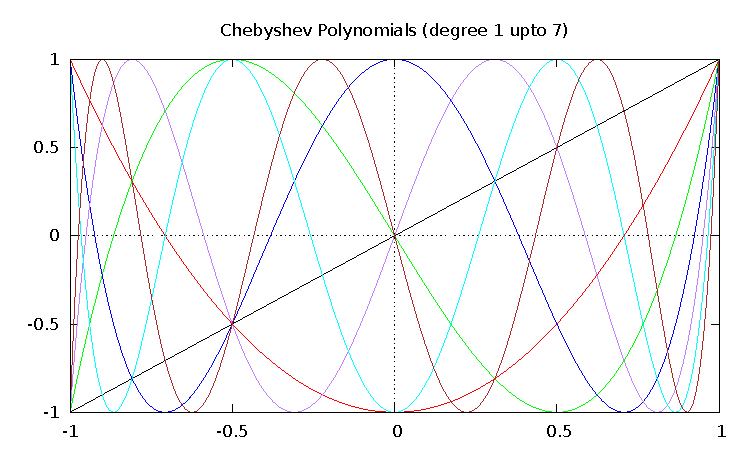
\includegraphics[width=4in]{example.pdf}

\subsection{Links to images and converting PDFs to high quality raster images}
\label{sec:org258244e}

Here we have a pretty graph (in a PNG file):

\begin{center}
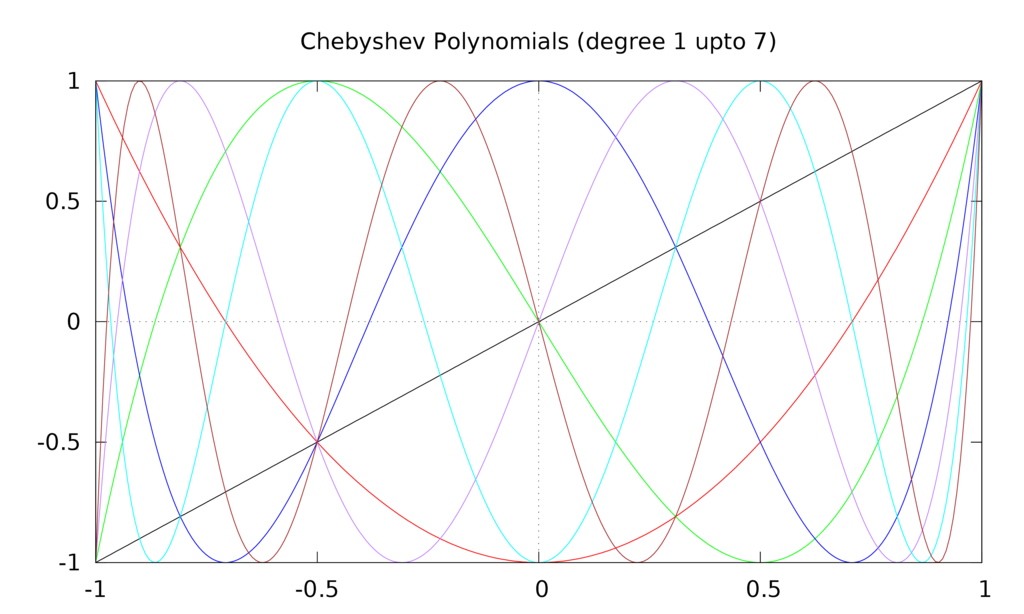
\includegraphics[width=.9\linewidth]{example.png}
\end{center}

The above file was generated from a high quality PDF file: \href{example.pdf}{example.pdf}. Note that the link in the previous sentence is a link in both HTML and \LaTeX{} because
the link has a 'display text' component.

The conversion was done like so:

\begin{verbatim}
convert -density 600 -resize 1024 -background white -flatten example.pdf example.png
\end{verbatim}

\section{Including external code}
\label{sec:org425d198}

Some Ruby code is the file \url{example.rb}.  It's contents are listed below:

\begin{verbatim}
#!/usr/local/bin/ruby

##
# @file      hello.rb
# @author    Mitch Richling <http://www.mitchr.me/>
# @Copyright Copyright 2006 by Mitch Richling.  All rights reserved.
# @brief     The classic hello world program the Ruby way.@EOL
# @Keywords  ruby example hello world
# @Std       Ruby 1.8
#
#            The methods puts, print, printf & putc are all in the IO
#            class as well so that they can be used to write to
#            different IO streams.  As used here, they write to
#            STDOUT.

puts("Hello, World!")

print("Hello, World!\n")

printf("Hello, World!\n")

STDOUT << "Hello, World!\n"

STDOUT.write("Hello, World!\n")

"Hello, World!\n".each_byte {|b| putc(b) }
\end{verbatim}

\section{Inline Code}
\label{sec:org239d8cb}

Here is a number, \texttt{\texttt{(* 2 3)}} \texttt{6}, that comes from a bit of elisp code.

\section{Code Blocks}
\label{sec:org8663c64}

\subsection{Text code blocks}
\label{sec:orga77156e}

Text code blocks can be used as a kind of verbatum environment instead of BEGIN\_EXAMPLE.

\begin{verbatim}
> Some Mail
>> Some More
>>> Even More
>>>> Even more
\end{verbatim}

\subsection{Email code blocks}
\label{sec:orgbc9a545}

This is nice because we get some highlighting for quoted e-mails and threads.

\begin{verbatim}
> Some Mail
>> Some More
>>> Even More
>>>> Even more
\end{verbatim}

\subsection{Emacs Lisp}
\label{sec:org75d4c68}

While you can use "value" insead of "output" for code blocks, it really is \textbf{very} usefull for Emacs Lisp.

\begin{verbatim}
(+ 1 2 3 5)
\end{verbatim}

\begin{verbatim}
11
\end{verbatim}

\subsection{Emacs Calc}
\label{sec:org2b2552f}

For more complex mathematical computations done with just Emacs (no outside tools) we can use calc.

\begin{verbatim}
deriv(3*x^2+log(x), x)
\end{verbatim}

\begin{verbatim}
6 x + 1 / x
\end{verbatim}

\subsection{Maxima}
\label{sec:org3bdb521}

For super complex math, we can use maxima.  

Here we see a  pretty printed result

\begin{verbatim}
programmode:false;
d:diff(3*x^2+log(x), x);
print(d);
\end{verbatim}

\begin{verbatim}
      1
6 x + - 
      x
\end{verbatim}

Same answer, but 2D printed

\begin{verbatim}
programmode:false;
display2d:false;
d:diff(3*x^2+log(x), x);
print(d);
\end{verbatim}

\begin{verbatim}
6*x+1/x 
\end{verbatim}

Lastly note we can also output things in \LaTeX{}, and get them rendered on export!

\begin{verbatim}
programmode:false;
d:diff(3*x^2+log(x), x);
tex(d);
\end{verbatim}

$$6\,x+{{1}\over{x}}$$

Another cool application is ot use the \texttt{fortran} function to have maxima spit out results in fortran syntax.

\subsection{Shells}
\label{sec:org458ae63}

\begin{verbatim}
date "+%Y-%m-%d %H:%M:%S"
\end{verbatim}

\begin{verbatim}
2020-07-21 16:27:29
\end{verbatim}

\subsection{Ruby}
\label{sec:org86b9900}

\begin{verbatim}
puts("HI MOM")
\end{verbatim}

\begin{verbatim}
HI MOM
\end{verbatim}

\subsection{Perl}
\label{sec:orgd9ae186}

\begin{verbatim}
print "HI MOM\n";
\end{verbatim}

\begin{verbatim}
HI MOM
\end{verbatim}

\section{Fancy Code Block Stuff}
\label{sec:orgadb7932}
\subsection{Generateing code}
\label{sec:org175b01c}

\begin{verbatim}
(cl-loop for f in '("foo" "bar")
         do (princ (message "mv %s %s.bak\n" f f)))
\end{verbatim}

\begin{verbatim}
mv foo foo.bak
mv bar bar.bak
\end{verbatim}

\subsection{Code links}
\label{sec:orgb0eaeec}

You can link to a target inside a code block: Visible Link Text

\begin{verbatim}
(cl-loop for f in '("foo" "bar")                       ;;      (foo)
         do (princ (message "mv %s %s.bak\n" f f)))
\end{verbatim}

You can remove the visable refrences from the source listings with the -r option in the babel header.  Otherwise they will appear in the listing -- fontlocked
white.

\subsection{Line Numbers}
\label{sec:orgd095d05}

This will include line numbers in the block when exported

\begin{verbatim}
(cl-loop for f in '("foo" "bar")
         do (princ (message "mv %s %s.bak\n" f f)))
\end{verbatim}

\section{dot}
\label{sec:org1eb5fd0}

Here we do not export the code, just the results -- as an image.  This results in a nice rendering.

\begin{verbatim}
graph {
 A -- B;
}
\end{verbatim}

\begin{center}
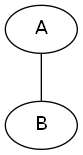
\includegraphics[width=.9\linewidth]{dotResult.png}
\end{center}

\section{R}
\label{sec:org099cc8d}

\subsection{Just run some R code in a new session}
\label{sec:orgf2a44bb}

\begin{verbatim}
print("HI MOM")
\end{verbatim}

\begin{verbatim}
[1] "HI MOM"
\end{verbatim}

\subsection{Access a table in this document as a data.frame}
\label{sec:orgdefcd96}

\begin{verbatim}
someData
\end{verbatim}

\begin{verbatim}
  factor.1 factor.2 value.1 value.2
1        a        z       1       5
2        a        x       2       6
3        a        y       3       7
4        b        x       4      NA
\end{verbatim}

\subsection{Output from R as a org-mode table}
\label{sec:org979f422}

\begin{verbatim}
someData
\end{verbatim}

\begin{center}
\begin{tabular}{llrr}
a & z & 1 & 5\\
a & x & 2 & 6\\
a & y & 3 & 7\\
b & x & 4 & nil\\
\end{tabular}
\end{center}

\subsection{Run some code in a R persistent session (the someData variable is available for later blocks)}
\label{sec:org1b86d59}
\begin{verbatim}
someData <- data.frame(a=1:10, b=rnorm(10))
print(someData)
\end{verbatim}

\begin{verbatim}
    a          b
1   1  1.2417875
2   2  0.8637138
3   3 -1.9440137
4   4 -0.3236072
5   5 -1.3049771
6   6 -1.3039629
7   7 -0.5288673
8   8  0.7139287
9   9  1.1919474
10 10  0.6513476
\end{verbatim}

\subsection{Use the someData variable in the session, and draw a graph.}
\label{sec:org7ad5a7c}

No speical org-mode stuff for graphics.  Just saved the output in files via R.  Add link text later.

\begin{verbatim}
g <- ggplot(someData, aes(x=a, y=b)) + geom_line()
ggsave("rOut1.png", width=8, height=6, dpi=100, units='in', plot=g);
ggsave("rOut1.pdf", width=8, height=6, dpi=600, units='in', plot=g);
\end{verbatim}

The graph:

\begin{center}
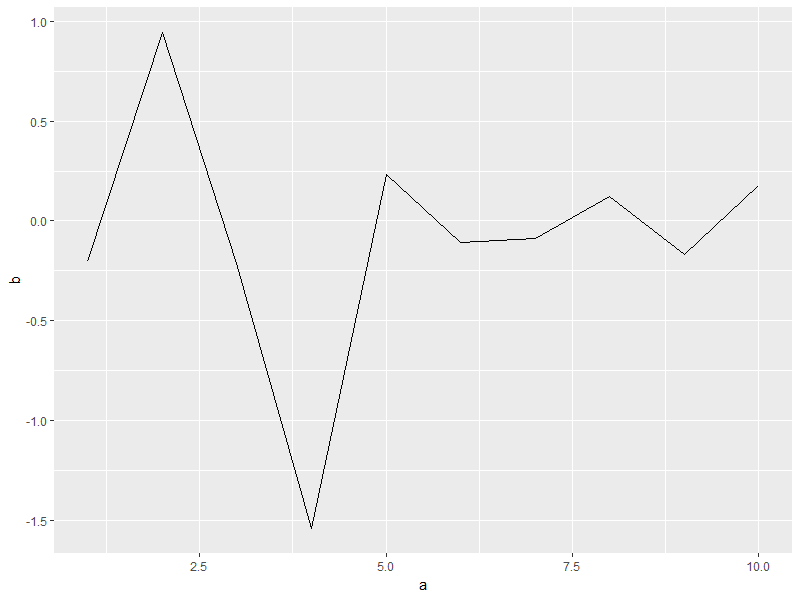
\includegraphics[width=.9\linewidth]{rOut1.png}
\end{center}

A high quality PDF version is \href{rOut1.pdf}{here} -- note the "here" is a link for both \LaTeX{} and HTML.

\subsection{We can use org-mode to make the file too.}
\label{sec:orgcd8870c}

Note: :session is required for this to work -- otherwise we must "print" the graphic.

\begin{verbatim}
ggplot(someData, aes(x=a, y=b)) + geom_line()
\end{verbatim}

\begin{center}
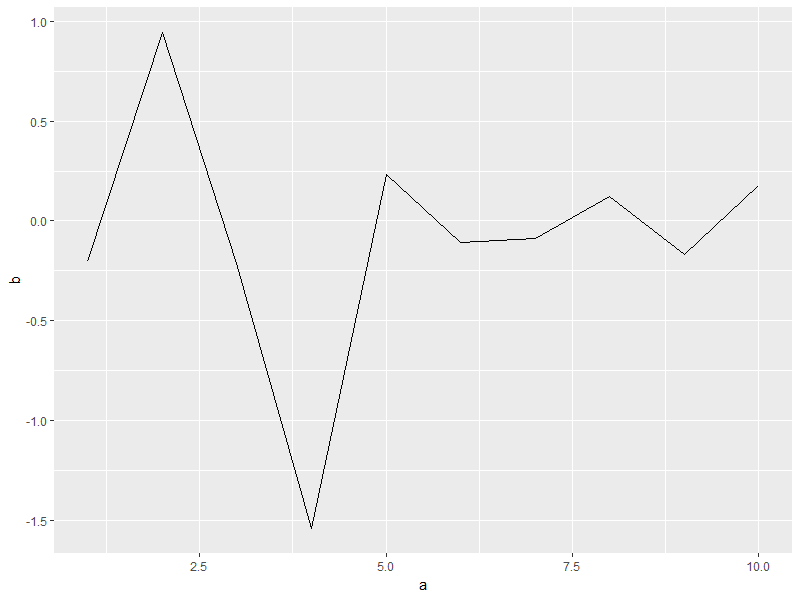
\includegraphics[width=.9\linewidth]{rOut1.png}
\end{center}

\subsection{And plotly works too}
\label{sec:org4951e9f}

Note the silent output -- we don't need the result, so we just don't print it.

\begin{verbatim}
library(plotly)
library(htmlwidgets)
data(diamonds, package = "ggplot2")
ggp <- ggplot(diamonds, aes(x = log(carat), y = log(price))) + geom_hex(bins = 100)
plp <- ggplotly(ggp)
saveWidget(plp, "examplePlotly.html", selfcontained=FALSE, libdir="examplePlotlyLib")
\end{verbatim}

\section{Reproduciblity}
\label{sec:orgc8994c6}

This section is here to help anyone wishing to reproduce the results above, or to understand the mechanics of how the results were obtained..

Reminder: All blocks in the entire tree can be evaluated with C-C C-V C-S

\subsection{FILES}
\label{sec:org6e96c64}

Documented in this section are (for each file in this archive):

\begin{itemize}
\item SHA1
\item Output from an 'ls -l' command
\item Output from the 'wc' command -- byte, word, and line counts
\end{itemize}

The use cases are two fold:

\begin{itemize}
\item Insure that the input data files being used are the same
\item Check if reproduced results match
\end{itemize}

Replace the \texttt{`find ./ -type f`} with a list of files and/or wildcards to explicitly select the desired files.

\begin{verbatim}
date
for c in wc 'openssl sha1' 'ls -l' ; do
    echo $c; $c `find ./ -type f`
done
\end{verbatim}

\begin{verbatim}
Wed, Jan 22, 2020 11:08:31 PM
wc
      0       1      30 ./.#genericOrgTemplate.org
     73      81    1268 ./auto/genericOrgTemplate.el
     23      79    3063 ./dotResult.png
    186     683   16335 ./example.pdf
   1316    7419  347721 ./example.png
     26      96     695 ./example.rb
     10      10     149 ./files_to_publish
     11      11     157 ./files_to_publish_before
   1366    5177   54165 ./genericOrgTemplate.html
   1371    5185   54236 ./genericOrgTemplate.html~
    636    2886   21429 ./genericOrgTemplate.org
    615    2736   20681 ./genericOrgTemplate.org~
   5312   13987  457794 ./genericOrgTemplate.pdf
    623    2019   17088 ./genericOrgTemplate.tex
     80     274    4458 ./rOut1.pdf
     45     328    7486 ./rOut1.png
     21     229    7185 ./rOut2.png
  11714   41201 1013940 total
openssl sha1
SHA1(./.#genericOrgTemplate.org)= 62941e0a5896f2b4efe7e63e97b054a866ec3f02
SHA1(./auto/genericOrgTemplate.el)= 1792aa6f454e97af4f40b729b55cba5f175fe622
SHA1(./dotResult.png)= 0aee67ef545690ac2edfacca997a2830bf52e5bd
SHA1(./example.pdf)= 32331c8ba2289b7b3c44b494c738ef0ad9973980
SHA1(./example.png)= d193ac9077e6616ee3d849184453195c414c49c9
SHA1(./example.rb)= ee55cdae5e8017b96fe18ab376356ff6d610ab78
SHA1(./files_to_publish)= f8b013770c45ea8efdf4eeb135e53023f756233d
SHA1(./files_to_publish_before)= f912ac87b274c3575fe7617f4d582abb75118784
SHA1(./genericOrgTemplate.html)= 5f171f9bb3c3b0cca8b45bfe3badb53c1b310c60
SHA1(./genericOrgTemplate.html~)= 1639270987f332dd9419256c9078385257bf3f52
SHA1(./genericOrgTemplate.org)= 98295573751daf0a7f77084b8d3c502fc7cb4f91
SHA1(./genericOrgTemplate.org~)= 7d1a924a6300d622abcf42fcad1660952b7b442e
SHA1(./genericOrgTemplate.pdf)= c1cb58664f48963eccab99496debd518f92a1a5d
SHA1(./genericOrgTemplate.tex)= d4982cfaeb44e15954aff17ac0977b2743c6a4ab
SHA1(./rOut1.pdf)= f165e5c93e05c20ec4264e7418dd620b120e77e5
SHA1(./rOut1.png)= 285f7b2b81e15fd96e4cc1d3fc7f6a0f0042baca
SHA1(./rOut2.png)= d6e8fd09c7a3bbbc7fbd1adab8325243e8d23fad
ls -l
-rw-r--r-- 1 richmit None     30 Jan 22 23:08 ./.#genericOrgTemplate.org
-rw-r--r-- 1 richmit None   1268 May 29  2016 ./auto/genericOrgTemplate.el
-rw-r--r-- 1 richmit None   3063 Jan 22 14:47 ./dotResult.png
-rw-r--r-- 1 richmit None  16335 May 30  2015 ./example.pdf
-rw-r--r-- 1 richmit None 347721 May 30  2015 ./example.png
-rwxr-xr-x 1 richmit None    695 May 30  2015 ./example.rb
-rw-r--r-- 1 richmit None    149 Jan 22 14:47 ./files_to_publish
-rw-r--r-- 1 richmit None    157 Jan 22 14:47 ./files_to_publish_before
-rw-r--r-- 1 richmit None  54165 Jan 22 23:08 ./genericOrgTemplate.html
-rw-r--r-- 1 richmit None  54236 Jan 22 23:05 ./genericOrgTemplate.html~
-rw-r--r-- 1 richmit None  21429 Jan 22 23:08 ./genericOrgTemplate.org
-rw-r--r-- 1 richmit None  20681 Jan 22 14:53 ./genericOrgTemplate.org~
-rw-r--r-- 1 richmit None 457794 May 29  2016 ./genericOrgTemplate.pdf
-rw-r--r-- 1 richmit None  17088 May 29  2016 ./genericOrgTemplate.tex
-rw-r--r-- 1 richmit None   4458 Jan 22 23:07 ./rOut1.pdf
-rw-r--r-- 1 richmit None   7486 Jan 22 23:07 ./rOut1.png
-rw-r--r-- 1 richmit None   7185 Jan 22 23:07 ./rOut2.png
\end{verbatim}

\subsection{ENVIRONMENT}
\label{sec:org0dd90a2}

The input files are only part of the reproduciblity equation.  It is also important to understand the tools and computational environment used for the
original analysis.  This section contains various bits of meta-data about the tools and system I used for this analysis.

\subsubsection{Embedded Ruby Version}
\label{sec:org47f9761}

\begin{verbatim}
puts(RUBY_VERSION)
\end{verbatim}

\begin{verbatim}
2.6.3
\end{verbatim}

\subsubsection{Embedded Perl Version}
\label{sec:org5f8e6fe}

\begin{verbatim}
print $]
\end{verbatim}

\begin{verbatim}
5.030000
\end{verbatim}

\subsubsection{Embedded R Information}
\label{sec:org60a83f1}

\paragraph{R version}
\label{sec:orgdedce00}

\begin{verbatim}
R.version
\end{verbatim}

\begin{verbatim}
               _                           
platform       x86_64-w64-mingw32          
arch           x86_64                      
os             mingw32                     
system         x86_64, mingw32             
status                                     
major          3                           
minor          5.3                         
year           2019                        
month          03                          
day            11                          
svn rev        76217                       
language       R                           
version.string R version 3.5.3 (2019-03-11)
nickname       Great Truth                 
\end{verbatim}

\paragraph{Session Information}
\label{sec:orgcb12abe}

\begin{verbatim}
sessionInfo()
\end{verbatim}

\begin{verbatim}
R version 3.5.3 (2019-03-11)
Platform: x86_64-w64-mingw32/x64 (64-bit)
Running under: Windows 10 x64 (build 18363)

Matrix products: default

locale:
[1] LC_COLLATE=English_United States.1252  LC_CTYPE=English_United States.1252    LC_MONETARY=English_United States.1252 LC_NUMERIC=C                           LC_TIME=English_United States.1252    

attached base packages:
[1] graphics  grDevices datasets  utils     grid      stats     methods   base     

other attached packages:
 [1] RevoUtils_11.0.3     RColorBrewer_1.1-2   reshape2_1.4.3       scales_1.0.0         ggplot2_3.1.1        tidyr_0.8.3          dplyr_0.8.0.1        data.table_1.12.2    gridExtra_2.3       
[10] jsonlite_1.5         knitr_1.22           lattice_0.20-38      RevoUtilsMath_11.0.0

loaded via a namespace (and not attached):
 [1] Rcpp_1.0.1       magrittr_1.5     tidyselect_0.2.5 munsell_0.5.0    colorspace_1.4-1 R6_2.3.0         rlang_0.3.4      stringr_1.4.0    plyr_1.8.4       tools_3.5.3      gtable_0.3.0    
[12] xfun_0.6         withr_2.1.2      lazyeval_0.2.2   assertthat_0.2.1 tibble_2.1.1     crayon_1.3.4     purrr_0.3.2      glue_1.3.1       stringi_1.4.3    compiler_3.5.3   pillar_1.3.1    
[23] pkgconfig_2.0.2 
\end{verbatim}

\paragraph{Loaded Package Versions}
\label{sec:org871f4cb}

\begin{verbatim}
installed.packages()[(loadedNamespaces()),c('Version', 'LibPath')]
\end{verbatim}

\begin{verbatim}
              Version   LibPath                                                                  
Rcpp          "1.0.1"   "c:/Users/richmit/Documents/R/win-library/x86_64-w64-mingw32-3.5.3/opkgs"
knitr         "1.22"    "c:/Users/richmit/Documents/R/win-library/x86_64-w64-mingw32-3.5.3/opkgs"
magrittr      "1.5"     "c:/Users/richmit/Documents/R/win-library/x86_64-w64-mingw32-3.5.3/opkgs"
grDevices     "3.5.3"   "C:/Program Files/Microsoft/R Open/R-3.5.3/library"                      
tidyselect    "0.2.5"   "c:/Users/richmit/Documents/R/win-library/x86_64-w64-mingw32-3.5.3/opkgs"
munsell       "0.5.0"   "c:/Users/richmit/Documents/R/win-library/x86_64-w64-mingw32-3.5.3/opkgs"
colorspace    "1.4-1"   "c:/Users/richmit/Documents/R/win-library/x86_64-w64-mingw32-3.5.3/opkgs"
lattice       "0.20-38" "C:/Program Files/Microsoft/R Open/R-3.5.3/library"                      
R6            "2.3.0"   "C:/Program Files/Microsoft/R Open/R-3.5.3/library"                      
rlang         "0.3.4"   "c:/Users/richmit/Documents/R/win-library/x86_64-w64-mingw32-3.5.3/opkgs"
RevoUtilsMath "11.0.0"  "C:/Program Files/Microsoft/R Open/R-3.5.3/library"                      
stringr       "1.4.0"   "c:/Users/richmit/Documents/R/win-library/x86_64-w64-mingw32-3.5.3/opkgs"
plyr          "1.8.4"   "c:/Users/richmit/Documents/R/win-library/x86_64-w64-mingw32-3.5.3/opkgs"
dplyr         "0.8.0.1" "c:/Users/richmit/Documents/R/win-library/x86_64-w64-mingw32-3.5.3/opkgs"
tools         "3.5.3"   "C:/Program Files/Microsoft/R Open/R-3.5.3/library"                      
utils         "3.5.3"   "C:/Program Files/Microsoft/R Open/R-3.5.3/library"                      
grid          "3.5.3"   "C:/Program Files/Microsoft/R Open/R-3.5.3/library"                      
data.table    "1.12.2"  "c:/Users/richmit/Documents/R/win-library/x86_64-w64-mingw32-3.5.3/opkgs"
gtable        "0.3.0"   "c:/Users/richmit/Documents/R/win-library/x86_64-w64-mingw32-3.5.3/opkgs"
xfun          "0.6"     "c:/Users/richmit/Documents/R/win-library/x86_64-w64-mingw32-3.5.3/opkgs"
withr         "2.1.2"   "c:/Users/richmit/Documents/R/win-library/x86_64-w64-mingw32-3.5.3/opkgs"
datasets      "3.5.3"   "C:/Program Files/Microsoft/R Open/R-3.5.3/library"                      
stats         "3.5.3"   "C:/Program Files/Microsoft/R Open/R-3.5.3/library"                      
lazyeval      "0.2.2"   "c:/Users/richmit/Documents/R/win-library/x86_64-w64-mingw32-3.5.3/opkgs"
assertthat    "0.2.1"   "c:/Users/richmit/Documents/R/win-library/x86_64-w64-mingw32-3.5.3/opkgs"
tibble        "2.1.1"   "c:/Users/richmit/Documents/R/win-library/x86_64-w64-mingw32-3.5.3/opkgs"
base          "3.5.3"   "C:/Program Files/Microsoft/R Open/R-3.5.3/library"                      
crayon        "1.3.4"   "c:/Users/richmit/Documents/R/win-library/x86_64-w64-mingw32-3.5.3/opkgs"
gridExtra     "2.3"     "c:/Users/richmit/Documents/R/win-library/x86_64-w64-mingw32-3.5.3/opkgs"
RColorBrewer  "1.1-2"   "c:/Users/richmit/Documents/R/win-library/x86_64-w64-mingw32-3.5.3/opkgs"
reshape2      "1.4.3"   "c:/Users/richmit/Documents/R/win-library/x86_64-w64-mingw32-3.5.3/opkgs"
purrr         "0.3.2"   "c:/Users/richmit/Documents/R/win-library/x86_64-w64-mingw32-3.5.3/opkgs"
ggplot2       "3.1.1"   "c:/Users/richmit/Documents/R/win-library/x86_64-w64-mingw32-3.5.3/opkgs"
tidyr         "0.8.3"   "c:/Users/richmit/Documents/R/win-library/x86_64-w64-mingw32-3.5.3/opkgs"
graphics      "3.5.3"   "C:/Program Files/Microsoft/R Open/R-3.5.3/library"                      
glue          "1.3.1"   "c:/Users/richmit/Documents/R/win-library/x86_64-w64-mingw32-3.5.3/opkgs"
stringi       "1.4.3"   "c:/Users/richmit/Documents/R/win-library/x86_64-w64-mingw32-3.5.3/opkgs"
compiler      "3.5.3"   "C:/Program Files/Microsoft/R Open/R-3.5.3/library"                      
pillar        "1.3.1"   "c:/Users/richmit/Documents/R/win-library/x86_64-w64-mingw32-3.5.3/opkgs"
methods       "3.5.3"   "C:/Program Files/Microsoft/R Open/R-3.5.3/library"                      
RevoUtils     "11.0.3"  "C:/Program Files/Microsoft/R Open/R-3.5.3/library"                      
scales        "1.0.0"   "c:/Users/richmit/Documents/R/win-library/x86_64-w64-mingw32-3.5.3/opkgs"
jsonlite      "1.5"     "C:/Program Files/Microsoft/R Open/R-3.5.3/library"                      
pkgconfig     "2.0.2"   "c:/Users/richmit/Documents/R/win-library/x86_64-w64-mingw32-3.5.3/opkgs"
\end{verbatim}

\subsubsection{Emacs Information}
\label{sec:orgc1c70a0}

\paragraph{Emacs Version}
\label{sec:org4ffb94c}

\begin{verbatim}
(emacs-version)
\end{verbatim}

\begin{verbatim}
"GNU Emacs 26.2 (build 1, x86_64-w64-mingw32)
 of 2019-06-03"
\end{verbatim}

\paragraph{org-mode Version}
\label{sec:org2325591}

\begin{verbatim}
org-version
\end{verbatim}

\begin{verbatim}
"9.1.14"
\end{verbatim}

\paragraph{ESS Version}
\label{sec:org1906236}

\begin{verbatim}
(ess-version)
\end{verbatim}

\begin{verbatim}
"ess-version: 18.10.3snapshot [elpa: 20200103.915] (loaded from c:/msys64/home/richmit/.emacs.d/elpa/ess-20200103.915/)"
\end{verbatim}

\paragraph{Process Environment}
\label{sec:orgd9c2f02}

\begin{verbatim}
process-environment
\end{verbatim}

\begin{verbatim}
("tmp=C:\\Users\\richmit\\AppData\\Local\\Temp" "temp=C:\\Users\\richmit\\AppData\\Local\\Temp" "WINDIR=C:\\WINDOWS" "VISIT_MPIEXEC=C:\\Program Files\\Microsoft MPI\\Bin\\mpiexec.exe" "VISITPLUGININSTPUB=C:\\Program Files\\LLNL\\VisIt 2.13.3" "VISITPLUGININSTPRI=C:\\Users\\richmit\\AppData\\Roaming\\LLNL\\VisIt" "VISITLOC=C:\\Program Files\\LLNL\\VisIt 2.13.3" "VISITARCHHOME=C:\\Program Files\\LLNL\\VisIt 2.13.3" "USERPROFILE=C:\\Users\\richmit" "USERNAME=richmit" "USERDOMAIN_ROAMINGPROFILE=HOFUD" "USERDOMAIN=HOFUD" "USER=richmit" "TMUX_PANE=%7" "TMUX=C:/msys64/home/richmit/tmp/tmux/sockets/0_hofud,441,0" "TMP=C:\\msys64\\tmp" "TEXINPUTS=.;C:\\msys64\\home\\richmit\\core\\texinputs;" "TERM=dumb" "TEMP=C:\\msys64\\tmp" "SYSTEMROOT=C:\\WINDOWS" "SYSTEMDRIVE=C:" "SHLVL=4" "SHELL=C:/msys64/usr/bin/zsh" "SESSIONNAME=Console" "SBCL_HOME=C:\\Program Files\\Steel Bank Common Lisp\\1.4.14\\" "ProgramW6432=C:\\Program Files" "ProgramFiles(x86)=C:\\Program Files (x86)" "ProgramData=C:\\ProgramData" "PWD=C:/msys64/home/richmit" "PUBLIC=C:\\Users\\Public" "PSModulePath=C:\\Program Files\\WindowsPowerShell\\Modules;C:\\WINDOWS\\system32\\WindowsPowerShell\\v1.0\\Modules" "PROGRAMFILES=C:\\Program Files" "PROCESSOR_REVISION=8e0a" "PROCESSOR_LEVEL=6" "PROCESSOR_IDENTIFIER=Intel64 Family 6 Model 142 Stepping 10, GenuineIntel" "PROCESSOR_ARCHITECTURE=AMD64" "PRINTER=Microsoft Print to PDF" "PKG_CONFIG_PATH=C:\\msys64\\mingw64\\lib\\pkgconfig;C:\\msys64\\mingw64\\share\\pkgconfig" "PATHEXT=.COM;.EXE;.BAT;.CMD;.VBS;.VBE;.JS;.JSE;.WSF;.WSH;.MSC" "PATH=.;C:\\msys64\\home\\richmit\\bin;C:\\texlive\\2018\\bin\\win32;C:\\msys64\\mingw64\\bin;C:\\msys64\\mingw32\\bin;C:\\msys64\\usr\\local\\bin;C:\\msys64\\mingw32\\sbin;C:\\msys64\\mingw32\\bin;C:\\msys64\\mingw64\\sbin;C:\\msys64\\mingw64\\bin;C:\\msys64\\usr\\sbin;C:\\msys64\\usr\\bin;C:\\msys64\\usr\\bin;C:\\Windows\\System32;C:\\Windows;C:\\Windows\\System32\\Wbem;C:\\Windows\\System32\\WindowsPowerShell\\v1.0\\" "PAGER=C:/msys64/usr/bin/less" "OneDriveConsumer=C:\\Users\\richmit\\OneDrive" "OneDrive=C:\\Users\\richmit\\OneDrive" "OS=Windows_NT" "ORIGINAL_TMP=C:/Users/richmit/AppData/Local/Temp" "ORIGINAL_TEMP=C:/Users/richmit/AppData/Local/Temp" "ORIGINAL_PATH=C:\\Windows\\System32;C:\\Windows;C:\\Windows\\System32\\Wbem;C:\\Windows\\System32\\WindowsPowerShell\\v1.0\\" "OLDPWD=C:/msys64/home/richmit/world/dotfiles/.emacs.d" "NUMBER_OF_PROCESSORS=8" "MYAPPS=C:/msys64/home/richmit/local" "MSYSTEM_PREFIX=C:/msys64/mingw64" "MSYSTEM_CHOST=x86_64-w64-mingw32" "MSYSTEM_CARCH=x86_64" "MSYSTEM=MINGW64" "MSYSCON=mintty.exe" "MSMPI_BIN=C:\\Program Files\\Microsoft MPI\\Bin\\" "MINGW_PREFIX=C:/msys64/mingw64" "MINGW_PACKAGE_PREFIX=mingw-w64-x86_64" "MINGW_CHOST=x86_64-w64-mingw32" "MANPATH=C:\\msys64\\usr\\share\\man;C:\\msys64\\mingw64\\share\\man;C:\\msys64\\mingw32\\share\\man" "LOGONSERVER=\\\\HOFUD" "LOGNAME=richmit" "LOCALAPPDATA=C:\\Users\\richmit\\AppData\\Local" "LANG=en_US.UTF-8" "INFOPATH=C:\\msys64\\usr\\share\\info;C:\\msys64\\mingw64\\share\\info;C:\\msys64\\mingw32\\share\\info" "IGNOREEOF=10" "HOSTNAME=hofud" "HOMEPATH=\\Users\\richmit" "HOMEDRIVE=C:" "HOME=C:\\msys64\\home\\richmit" "FPS_BROWSER_USER_PROFILE_STRING=Default" "FPS_BROWSER_APP_PROFILE_STRING=Internet Explorer" "EDITOR=C:/msys64/usr/bin/vim" "DriverData=C:\\Windows\\System32\\Drivers\\DriverData" "CommonProgramW6432=C:\\Program Files\\Common Files" "CommonProgramFiles(x86)=C:\\Program Files (x86)\\Common Files" "CONFIG_SITE=C:/msys64/mingw64/etc/config.site" "COMSPEC=C:\\WINDOWS\\system32\\cmd.exe" "COMPUTERNAME=HOFUD" "COMMONPROGRAMFILES=C:\\Program Files\\Common Files" "COMMONAPPDATA=C:\\ProgramData" "BIBINPUTS=.;" "APPDATA=C:\\Users\\richmit\\AppData\\Roaming" "ALLUSERSPROFILE=C:\\ProgramData" "ACLOCAL_PATH=C:\\msys64\\mingw64\\share\\aclocal;C:\\msys64\\usr\\share\\aclocal" "!;=;\\")
\end{verbatim}

\paragraph{System Type}
\label{sec:orgc0583de}

\begin{verbatim}
system-type
\end{verbatim}

\begin{verbatim}
windows-nt
\end{verbatim}

\paragraph{System Configuration}
\label{sec:org4c341fa}

\begin{verbatim}
system-configuration
\end{verbatim}

\begin{verbatim}
"x86_64-w64-mingw32"
\end{verbatim}

\subsubsection{System Information}
\label{sec:org38a3a1f}

\begin{verbatim}
for e in date whoami groups id hostname domainname dnsdomainname 'ifconfig -a' 'uname -a' 'openssl version' locale 'ldconfig -p' 'dpkg-query -l'; do
  c=`echo $e | awk '{print $1}'`;
  if hash $c 1>/dev/null 2>/dev/null; then 
    ruby -e 'puts("="*90)'
    echo $e
    sh -c "$e"
  fi
done
\end{verbatim}

\begin{verbatim}
==========================================================================================
date
Wed, Jan 22, 2020 11:08:43 PM
==========================================================================================
whoami
richmit
==========================================================================================
groups
None Users Performance Log Users INTERACTIVE CONSOLE LOGON Authenticated Users This Organization Local account CurrentSession LOCAL NTLM Authentication Medium Mandatory Level
==========================================================================================
id
uid=197609(richmit) gid=197121(None) groups=197121(None),545(Users),559(Performance Log Users),4(INTERACTIVE),66049(CONSOLE LOGON),11(Authenticated Users),15(This Organization),113(Local account),4095(CurrentSession),66048(LOCAL),262154(NTLM Authentication),401408(Medium Mandatory Level)
==========================================================================================
hostname
hofud
==========================================================================================
dnsdomainname
==========================================================================================
uname -a
MINGW64_NT-10.0-18363 hofud 3.0.7-338.x86_64 2019-07-11 10:58 UTC x86_64 Msys
==========================================================================================
openssl version
OpenSSL 1.1.1c  28 May 2019
==========================================================================================
locale
LANG=en_US.UTF-8
LC_CTYPE="en_US.UTF-8"
LC_NUMERIC="en_US.UTF-8"
LC_TIME="en_US.UTF-8"
LC_COLLATE="en_US.UTF-8"
LC_MONETARY="en_US.UTF-8"
LC_MESSAGES="en_US.UTF-8"
LC_ALL=
\end{verbatim}

\subsubsection{Command Line Tool Information}
\label{sec:org4444219}

\begin{verbatim}
for e in gcc g++ gfortran                               \
         wc ls grep sed awk cut sort uniq               \
         bash ksh tcsh dash csh sh zsh                  \
         vi vim emacs em                                \
         ruby ruby1.8 ruby2 python3 python2 perl        \
         gnuplot maxima octave M2 gap julia R           \
         qtiplot ggobi                                  \
         povray                                         \
         openscad xcircuit                              \
         convert pqiv import display                    \
         gs pdftex pdflatex tex latex dvips             \
         sbcl clisp ecl ccl                             \
         diff diff3 patch merge                         \
         sqlite3 mysqld                                 \
         paraview visit                                 \
         grass                                          \
         tar gzip bzip2 ; do
  ruby -e 'puts("="*90)'
  echo "Tool: $e"
  if hash $e 1>/dev/null 2>/dev/null; then 
    CPH=`which $e`
    if [ -n "$CPH" -a -e "$CPH" ] ; then
      echo $CPH    | sed 's/^/  Path: /'
      ls -ld $CPH  | sed 's/^/  ls-l: /'
      $e --version | sed 's/^/  Ver:  /'
    else
      echo "  Unable to locate (which): $e"
    fi
  else
    echo "  Unable to locate (hash): $e"
  fi
done
ruby -e 'puts("="*90)'
\end{verbatim}

\begin{verbatim}
==========================================================================================
Tool: gcc
  Path: /mingw64/bin/gcc
  ls-l: -rwxr-xr-x 1 richmit None 2137193 Aug 12 05:14 /mingw64/bin/gcc
  Ver:  gcc.exe (Rev1, Built by MSYS2 project) 9.2.0
  Ver:  Copyright (C) 2019 Free Software Foundation, Inc.
  Ver:  This is free software; see the source for copying conditions.  There is NO
  Ver:  warranty; not even for MERCHANTABILITY or FITNESS FOR A PARTICULAR PURPOSE.
  Ver:  
==========================================================================================
Tool: g++
  Path: /mingw64/bin/g++
  ls-l: -rwxr-xr-x 1 richmit None 2139753 Aug 12 05:14 /mingw64/bin/g++
  Ver:  g++.exe (Rev1, Built by MSYS2 project) 9.2.0
  Ver:  Copyright (C) 2019 Free Software Foundation, Inc.
  Ver:  This is free software; see the source for copying conditions.  There is NO
  Ver:  warranty; not even for MERCHANTABILITY or FITNESS FOR A PARTICULAR PURPOSE.
  Ver:  
==========================================================================================
Tool: gfortran
  Path: /mingw64/bin/gfortran
  ls-l: -rwxr-xr-x 1 richmit None 2139753 Aug 12 05:14 /mingw64/bin/gfortran
  Ver:  GNU Fortran (Rev1, Built by MSYS2 project) 9.2.0
  Ver:  Copyright (C) 2019 Free Software Foundation, Inc.
  Ver:  This is free software; see the source for copying conditions.  There is NO
  Ver:  warranty; not even for MERCHANTABILITY or FITNESS FOR A PARTICULAR PURPOSE.
  Ver:  
==========================================================================================
Tool: wc
  Path: /usr/bin/wc
  ls-l: -rwxr-xr-x 1 richmit None 42594 Apr 25  2019 /usr/bin/wc
  Ver:  wc (GNU coreutils) 8.31
  Ver:  Copyright (C) 2019 Free Software Foundation, Inc.
  Ver:  License GPLv3+: GNU GPL version 3 or later <https://gnu.org/licenses/gpl.html>.
  Ver:  This is free software: you are free to change and redistribute it.
  Ver:  There is NO WARRANTY, to the extent permitted by law.
  Ver:  
  Ver:  Written by Paul Rubin and David MacKenzie.
==========================================================================================
Tool: ls
  Path: /usr/bin/ls
  ls-l: -rwxr-xr-x 1 richmit None 139682 Apr 25  2019 /usr/bin/ls
  Ver:  ls (GNU coreutils) 8.31
  Ver:  Copyright (C) 2019 Free Software Foundation, Inc.
  Ver:  License GPLv3+: GNU GPL version 3 or later <https://gnu.org/licenses/gpl.html>.
  Ver:  This is free software: you are free to change and redistribute it.
  Ver:  There is NO WARRANTY, to the extent permitted by law.
  Ver:  
  Ver:  Written by Richard M. Stallman and David MacKenzie.
==========================================================================================
Tool: grep
  Path: /usr/bin/grep
  ls-l: -rwxr-xr-x 1 richmit None 210195 Dec  5  2018 /usr/bin/grep
  Ver:  grep (GNU grep) 3.0
  Ver:  Copyright (C) 2017 Free Software Foundation, Inc.
  Ver:  License GPLv3+: GNU GPL version 3 or later <http://gnu.org/licenses/gpl.html>.
  Ver:  This is free software: you are free to change and redistribute it.
  Ver:  There is NO WARRANTY, to the extent permitted by law.
  Ver:  
  Ver:  Written by Mike Haertel and others, see <http://git.sv.gnu.org/cgit/grep.git/tree/AUTHORS>.
==========================================================================================
Tool: sed
  Path: /usr/bin/sed
  ls-l: -rwxr-xr-x 1 richmit None 172307 Dec 26  2018 /usr/bin/sed
  Ver:  sed (GNU sed) 4.7
  Ver:  Copyright (C) 2018 Free Software Foundation, Inc.
  Ver:  License GPLv3+: GNU GPL version 3 or later <https://gnu.org/licenses/gpl.html>.
  Ver:  This is free software: you are free to change and redistribute it.
  Ver:  There is NO WARRANTY, to the extent permitted by law.
  Ver:  
  Ver:  Written by Jay Fenlason, Tom Lord, Ken Pizzini,
  Ver:  Paolo Bonzini, Jim Meyering, and Assaf Gordon.
  Ver:  GNU sed home page: <https://www.gnu.org/software/sed/>.
  Ver:  General help using GNU software: <https://www.gnu.org/gethelp/>.
  Ver:  E-mail bug reports to: <bug-sed@gnu.org>.
==========================================================================================
Tool: awk
  Path: /usr/bin/awk
  ls-l: -rwxr-xr-x 1 richmit None 626954 Jun 24  2019 /usr/bin/awk
  Ver:  GNU Awk 5.0.1, API: 2.0 (GNU MPFR 4.0.2, GNU MP 6.1.2)
  Ver:  Copyright (C) 1989, 1991-2019 Free Software Foundation.
  Ver:  
  Ver:  This program is free software; you can redistribute it and/or modify
  Ver:  it under the terms of the GNU General Public License as published by
  Ver:  the Free Software Foundation; either version 3 of the License, or
  Ver:  (at your option) any later version.
  Ver:  
  Ver:  This program is distributed in the hope that it will be useful,
  Ver:  but WITHOUT ANY WARRANTY; without even the implied warranty of
  Ver:  MERCHANTABILITY or FITNESS FOR A PARTICULAR PURPOSE.  See the
  Ver:  GNU General Public License for more details.
  Ver:  
  Ver:  You should have received a copy of the GNU General Public License
  Ver:  along with this program. If not, see http://www.gnu.org/licenses/.
==========================================================================================
Tool: cut
  Path: /usr/bin/cut
  ls-l: -rwxr-xr-x 1 richmit None 42378 Apr 25  2019 /usr/bin/cut
  Ver:  cut (GNU coreutils) 8.31
  Ver:  Copyright (C) 2019 Free Software Foundation, Inc.
  Ver:  License GPLv3+: GNU GPL version 3 or later <https://gnu.org/licenses/gpl.html>.
  Ver:  This is free software: you are free to change and redistribute it.
  Ver:  There is NO WARRANTY, to the extent permitted by law.
  Ver:  
  Ver:  Written by David M. Ihnat, David MacKenzie, and Jim Meyering.
==========================================================================================
Tool: sort
  Path: /usr/bin/sort
  ls-l: -rwxr-xr-x 1 richmit None 106313 Apr 25  2019 /usr/bin/sort
  Ver:  sort (GNU coreutils) 8.31
  Ver:  Copyright (C) 2019 Free Software Foundation, Inc.
  Ver:  License GPLv3+: GNU GPL version 3 or later <https://gnu.org/licenses/gpl.html>.
  Ver:  This is free software: you are free to change and redistribute it.
  Ver:  There is NO WARRANTY, to the extent permitted by law.
  Ver:  
  Ver:  Written by Mike Haertel and Paul Eggert.
==========================================================================================
Tool: uniq
  Path: /usr/bin/uniq
  ls-l: -rwxr-xr-x 1 richmit None 42325 Apr 25  2019 /usr/bin/uniq
  Ver:  uniq (GNU coreutils) 8.31
  Ver:  Copyright (C) 2019 Free Software Foundation, Inc.
  Ver:  License GPLv3+: GNU GPL version 3 or later <https://gnu.org/licenses/gpl.html>.
  Ver:  This is free software: you are free to change and redistribute it.
  Ver:  There is NO WARRANTY, to the extent permitted by law.
  Ver:  
  Ver:  Written by Richard M. Stallman and David MacKenzie.
==========================================================================================
Tool: bash
  Path: /usr/local/bin/bash
  ls-l: lrwxrwxrwx 1 richmit None 17 Dec 28  2018 /usr/local/bin/bash -> /usr/bin/bash.exe
  Ver:  GNU bash, version 4.4.23(1)-release (x86_64-pc-msys)
  Ver:  Copyright (C) 2016 Free Software Foundation, Inc.
  Ver:  License GPLv3+: GNU GPL version 3 or later <http://gnu.org/licenses/gpl.html>
  Ver:  
  Ver:  This is free software; you are free to change and redistribute it.
  Ver:  There is NO WARRANTY, to the extent permitted by law.
==========================================================================================
Tool: ksh
  Unable to locate (hash): ksh
==========================================================================================
Tool: tcsh
  Unable to locate (hash): tcsh
==========================================================================================
Tool: dash
  Path: /usr/bin/dash
  ls-l: -rwxr-xr-x 1 richmit None 104553 Jun 21  2018 /usr/bin/dash
==========================================================================================
Tool: csh
  Unable to locate (hash): csh
==========================================================================================
Tool: sh
  Path: /usr/bin/sh
  ls-l: -rwxr-xr-x 1 richmit None 1971272 Oct 30  2018 /usr/bin/sh
  Ver:  GNU bash, version 4.4.23(1)-release (x86_64-pc-msys)
  Ver:  Copyright (C) 2016 Free Software Foundation, Inc.
  Ver:  License GPLv3+: GNU GPL version 3 or later <http://gnu.org/licenses/gpl.html>
  Ver:  
  Ver:  This is free software; you are free to change and redistribute it.
  Ver:  There is NO WARRANTY, to the extent permitted by law.
==========================================================================================
Tool: vi
  Unable to locate (hash): vi
==========================================================================================
Tool: vim
  Path: /usr/bin/vim
  ls-l: -rwxr-xr-x 1 richmit None 2704119 Jul 30 06:28 /usr/bin/vim
  Ver:  VIM - Vi IMproved 8.1 (2018 May 18, compiled Jul 30 2019 11:28:50)
  Ver:  Included patches: 1-1777
  Ver:  Compiled by <alexpux@gmail.com>
  Ver:  Huge version without GUI.  Features included (+) or not (-):
  Ver:  +acl               -farsi             -mouse_sysmouse    -tag_any_white
  Ver:  +arabic            +file_in_path      +mouse_urxvt       -tcl
  Ver:  +autocmd           +find_in_path      +mouse_xterm       +termguicolors
  Ver:  +autochdir         +float             +multi_byte        +terminal
  Ver:  -autoservername    +folding           +multi_lang        +terminfo
  Ver:  -balloon_eval      -footer            -mzscheme          +termresponse
  Ver:  +balloon_eval_term +fork()            +netbeans_intg     +textobjects
  Ver:  -browse            +gettext           +num64             +textprop
  Ver:  ++builtin_terms    -hangul_input      +packages          +timers
  Ver:  +byte_offset       +iconv             +path_extra        +title
  Ver:  +channel           +insert_expand     +perl/dyn          -toolbar
  Ver:  +cindent           +job               +persistent_undo   +user_commands
  Ver:  -clientserver      +jumplist          +postscript        +vartabs
  Ver:  +clipboard         +keymap            +printer           +vertsplit
  Ver:  +cmdline_compl     +lambda            +profile           +virtualedit
  Ver:  +cmdline_hist      +langmap           +python/dyn        +visual
  Ver:  +cmdline_info      +libcall           +python3/dyn       +visualextra
  Ver:  +comments          +linebreak         +quickfix          +viminfo
  Ver:  +conceal           +lispindent        +reltime           +vreplace
  Ver:  +cryptv            +listcmds          +rightleft         +wildignore
  Ver:  +cscope            +localmap          +ruby/dyn          +wildmenu
  Ver:  +cursorbind        -lua               +scrollbind        +windows
  Ver:  +cursorshape       +menu              +signs             +writebackup
  Ver:  +dialog_con        +mksession         +smartindent       -X11
  Ver:  +diff              +modify_fname      -sound             -xfontset
  Ver:  +digraphs          +mouse             +spell             -xim
  Ver:  -dnd               -mouseshape        +startuptime       -xpm
  Ver:  -ebcdic            +mouse_dec         +statusline        -xsmp
  Ver:  +emacs_tags        -mouse_gpm         -sun_workshop      -xterm_clipboard
  Ver:  +eval              -mouse_jsbterm     +syntax            -xterm_save
  Ver:  +ex_extra          +mouse_netterm     +tag_binary        
  Ver:  +extra_search      +mouse_sgr         -tag_old_static    
  Ver:     system vimrc file: "/etc/vimrc"
  Ver:       user vimrc file: "$HOME/.vimrc"
  Ver:   2nd user vimrc file: "~/.vim/vimrc"
  Ver:        user exrc file: "$HOME/.exrc"
  Ver:         defaults file: "$VIMRUNTIME/defaults.vim"
  Ver:    fall-back for $VIM: "/etc"
  Ver:   f-b for $VIMRUNTIME: "/usr/share/vim/vim81"
  Ver:  Compilation: gcc -c -I. -Iproto -DHAVE_CONFIG_H   -I/usr/include/ncursesw  -march=x86-64 -mtune=generic -O2 -pipe -U_FORTIFY_SOURCE -D_FORTIFY_SOURCE=1       
  Ver:  Linking: gcc   -L. -pipe -fstack-protector-strong -pipe -Wl,--as-needed -o vim.exe        -lm -lelf    -lncursesw -liconv -lacl -lintl   -Wl,--enable-auto-import -Wl,--export-all-symbols -Wl,--enable-auto-image-base -fstack-protector-strong  -L/usr/lib/perl5/core_perl/CORE -lperl -lpthread -ldl -lcrypt        
==========================================================================================
Tool: emacs
  Path: /home/richmit/bin/emacs
  ls-l: -rwxr-xr-x 1 richmit None 8175 Dec 28  2018 /home/richmit/bin/emacs
  Ver:  GNU Emacs 26.2
  Ver:  Copyright (C) 2019 Free Software Foundation, Inc.
  Ver:  GNU Emacs comes with ABSOLUTELY NO WARRANTY.
  Ver:  You may redistribute copies of GNU Emacs
  Ver:  under the terms of the GNU General Public License.
  Ver:  For more information about these matters, see the file named COPYING.
==========================================================================================
Tool: em
  Path: /home/richmit/bin/em
  ls-l: -rwxr-xr-x 1 richmit None 8175 Dec 28  2018 /home/richmit/bin/em
  Ver:  GNU Emacs 26.2
  Ver:  Copyright (C) 2019 Free Software Foundation, Inc.
  Ver:  GNU Emacs comes with ABSOLUTELY NO WARRANTY.
  Ver:  You may redistribute copies of GNU Emacs
  Ver:  under the terms of the GNU General Public License.
  Ver:  For more information about these matters, see the file named COPYING.
==========================================================================================
Tool: ruby
  Path: /home/richmit/bin/ruby
  ls-l: -rwxr-xr-x 1 richmit None 8175 Jan  8  2019 /home/richmit/bin/ruby
  Ver:  ruby 2.6.3p62 (2019-04-16 revision 67580) [x64-mingw32]
==========================================================================================
Tool: ruby1.8
  Unable to locate (hash): ruby1.8
==========================================================================================
Tool: ruby2
  Unable to locate (hash): ruby2
==========================================================================================
Tool: python3
  Path: /home/richmit/bin/python3
  ls-l: -rwxr-xr-x 1 richmit None 8175 Dec 28  2018 /home/richmit/bin/python3
  Ver:  Python 3.7.4
==========================================================================================
Tool: python2
  Path: /home/richmit/bin/python2
  ls-l: -rwxr-xr-x 1 richmit None 8175 Dec 28  2018 /home/richmit/bin/python2
==========================================================================================
Tool: perl
  Path: /home/richmit/bin/perl
  ls-l: -rwxr-xr-x 1 richmit None 8175 Dec 28  2018 /home/richmit/bin/perl
  Ver:  
  Ver:  This is perl 5, version 30, subversion 0 (v5.30.0) built for x86_64-msys-thread-multi
  Ver:  
  Ver:  Copyright 1987-2019, Larry Wall
  Ver:  
  Ver:  Perl may be copied only under the terms of either the Artistic License or the
  Ver:  GNU General Public License, which may be found in the Perl 5 source kit.
  Ver:  
  Ver:  Complete documentation for Perl, including FAQ lists, should be found on
  Ver:  this system using "man perl" or "perldoc perl".  If you have access to the
  Ver:  Internet, point your browser at http://www.perl.org/, the Perl Home Page.
  Ver:  
==========================================================================================
Tool: gnuplot
  Path: /mingw64/bin/gnuplot
  ls-l: -rwxr-xr-x 1 richmit None 1942622 Jul 23  2019 /mingw64/bin/gnuplot
  Ver:  gnuplot 5.2 patchlevel 7
==========================================================================================
Tool: maxima
  Path: /home/richmit/bin/maxima
  ls-l: -rwxr-xr-x 1 richmit None 8175 Dec 28  2018 /home/richmit/bin/maxima
  Ver:  ERROR: Application not found: maxima
==========================================================================================
Tool: octave
  Unable to locate (hash): octave
==========================================================================================
Tool: M2
  Unable to locate (hash): M2
==========================================================================================
Tool: gap
  Unable to locate (hash): gap
==========================================================================================
Tool: julia
  Unable to locate (hash): julia
==========================================================================================
Tool: R
  Unable to locate (hash): R
==========================================================================================
Tool: qtiplot
  Unable to locate (hash): qtiplot
==========================================================================================
Tool: ggobi
  Unable to locate (hash): ggobi
==========================================================================================
Tool: povray
  Unable to locate (hash): povray
==========================================================================================
Tool: openscad
  Unable to locate (hash): openscad
==========================================================================================
Tool: xcircuit
  Unable to locate (hash): xcircuit
==========================================================================================
Tool: convert
  Path: /mingw64/bin/convert
  ls-l: -rwxr-xr-x 1 richmit None 24367 Jul 12  2019 /mingw64/bin/convert
  Ver:  Version: ImageMagick 7.0.8-53 Q16 x86_64 2019-07-12 https://imagemagick.org
  Ver:  Copyright: © 1999-2019 ImageMagick Studio LLC
  Ver:  License: https://imagemagick.org/script/license.php
  Ver:  Features: Cipher DPC HDRI Modules OpenCL OpenMP(4.5) 
  Ver:  Delegates (built-in): bzlib cairo djvu fftw flif fontconfig freetype gslib gvc heic jbig jng jp2 jpeg lcms lqr ltdl lzma openexr pangocairo png ps raqm raw rsvg tiff webp wmf xml zlib
==========================================================================================
Tool: pqiv
  Unable to locate (hash): pqiv
==========================================================================================
Tool: import
  Path: /mingw64/bin/import
  ls-l: -rwxr-xr-x 1 richmit None 24367 Jul 12  2019 /mingw64/bin/import
  Ver:  Version: ImageMagick 7.0.8-53 Q16 x86_64 2019-07-12 https://imagemagick.org
  Ver:  Copyright: © 1999-2019 ImageMagick Studio LLC
  Ver:  License: https://imagemagick.org/script/license.php
  Ver:  Features: Cipher DPC HDRI Modules OpenCL OpenMP(4.5) 
  Ver:  Delegates (built-in): bzlib cairo djvu fftw flif fontconfig freetype gslib gvc heic jbig jng jp2 jpeg lcms lqr ltdl lzma openexr pangocairo png ps raqm raw rsvg tiff webp wmf xml zlib
  Ver:  Usage: import.exe [options ...] [ file ]
  Ver:  
  Ver:  Image Settings:
  Ver:    -adjoin              join images into a single multi-image file
  Ver:    -border              include window border in the output image
  Ver:    -channel type        apply option to select image channels
  Ver:    -colorspace type     alternate image colorspace
  Ver:    -comment string      annotate image with comment
  Ver:    -compress type       type of pixel compression when writing the image
  Ver:    -define format:option
  Ver:                         define one or more image format options
  Ver:    -density geometry    horizontal and vertical density of the image
  Ver:    -depth value         image depth
  Ver:    -descend             obtain image by descending window hierarchy
  Ver:    -display server      X server to contact
  Ver:    -dispose method      layer disposal method
  Ver:    -dither method       apply error diffusion to image
  Ver:    -delay value         display the next image after pausing
  Ver:    -encipher filename   convert plain pixels to cipher pixels
  Ver:    -endian type         endianness (MSB or LSB) of the image
  Ver:    -encoding type       text encoding type
  Ver:    -filter type         use this filter when resizing an image
  Ver:    -format "string"     output formatted image characteristics
  Ver:    -frame               include window manager frame
  Ver:    -gravity direction   which direction to gravitate towards
  Ver:    -identify            identify the format and characteristics of the image
  Ver:    -interlace type      None, Line, Plane, or Partition
  Ver:    -interpolate method  pixel color interpolation method
  Ver:    -label string        assign a label to an image
  Ver:    -limit type value    Area, Disk, Map, or Memory resource limit
  Ver:    -monitor             monitor progress
  Ver:    -page geometry       size and location of an image canvas
  Ver:    -pause seconds       seconds delay between snapshots
  Ver:    -pointsize value     font point size
  Ver:    -quality value       JPEG/MIFF/PNG compression level
  Ver:    -quiet               suppress all warning messages
  Ver:    -regard-warnings     pay attention to warning messages
  Ver:    -repage geometry     size and location of an image canvas
  Ver:    -respect-parentheses settings remain in effect until parenthesis boundary
  Ver:    -sampling-factor geometry
  Ver:                         horizontal and vertical sampling factor
  Ver:    -scene value         image scene number
  Ver:    -screen              select image from root window
  Ver:    -seed value          seed a new sequence of pseudo-random numbers
  Ver:    -set property value  set an image property
  Ver:    -silent              operate silently, i.e. don't ring any bells 
  Ver:    -snaps value         number of screen snapshots
  Ver:    -support factor      resize support: > 1.0 is blurry, < 1.0 is sharp
  Ver:    -synchronize         synchronize image to storage device
  Ver:    -taint               declare the image as modified
  Ver:    -transparent-color color
  Ver:                         transparent color
  Ver:    -treedepth value     color tree depth
  Ver:    -verbose             print detailed information about the image
  Ver:    -virtual-pixel method
  Ver:                         Constant, Edge, Mirror, or Tile
  Ver:    -window id           select window with this id or name
  Ver:                         root selects whole screen
  Ver:  
  Ver:  Image Operators:
  Ver:    -annotate geometry text
  Ver:                         annotate the image with text
  Ver:    -colors value        preferred number of colors in the image
  Ver:    -crop geometry       preferred size and location of the cropped image
  Ver:    -encipher filename   convert plain pixels to cipher pixels
  Ver:    -geometry geometry   preferred size or location of the image
  Ver:    -help                print program options
  Ver:    -monochrome          transform image to black and white
  Ver:    -negate              replace every pixel with its complementary color 
  Ver:    -quantize colorspace reduce colors in this colorspace
  Ver:    -resize geometry     resize the image
  Ver:    -rotate degrees      apply Paeth rotation to the image
  Ver:    -strip               strip image of all profiles and comments
  Ver:    -thumbnail geometry  create a thumbnail of the image
  Ver:    -transparent color   make this color transparent within the image
  Ver:    -trim                trim image edges
  Ver:    -type type           image type
  Ver:  
  Ver:  Miscellaneous Options:
  Ver:    -debug events        display copious debugging information
  Ver:    -help                print program options
  Ver:    -list type           print a list of supported option arguments
  Ver:    -log format          format of debugging information
  Ver:    -version             print version information
  Ver:  
  Ver:  By default, 'file' is written in the MIFF image format.  To
  Ver:  specify a particular image format, precede the filename with an image
  Ver:  format name and a colon (i.e. ps:image) or specify the image type as
  Ver:  the filename suffix (i.e. image.ps).  Specify 'file' as '-' for
  Ver:  standard input or output.
==========================================================================================
Tool: display
  Path: /mingw64/bin/display
  ls-l: -rwxr-xr-x 1 richmit None 24367 Jul 12  2019 /mingw64/bin/display
  Ver:  Version: ImageMagick 7.0.8-53 Q16 x86_64 2019-07-12 https://imagemagick.org
  Ver:  Copyright: © 1999-2019 ImageMagick Studio LLC
  Ver:  License: https://imagemagick.org/script/license.php
  Ver:  Features: Cipher DPC HDRI Modules OpenCL OpenMP(4.5) 
  Ver:  Delegates (built-in): bzlib cairo djvu fftw flif fontconfig freetype gslib gvc heic jbig jng jp2 jpeg lcms lqr ltdl lzma openexr pangocairo png ps raqm raw rsvg tiff webp wmf xml zlib
  Ver:  Usage: display.exe [options ...] file [ [options ...] file ...]
  Ver:  
  Ver:  Image Settings:
  Ver:    -alpha option        on, activate, off, deactivate, set, opaque, copy
  Ver:                         transparent, extract, background, or shape
  Ver:    -antialias           remove pixel-aliasing
  Ver:    -authenticate password
  Ver:                         decipher image with this password
  Ver:    -backdrop            display image centered on a backdrop
  Ver:    -channel type        apply option to select image channels
  Ver:    -colormap type       Shared or Private
  Ver:    -colorspace type     alternate image colorspace
  Ver:    -comment string      annotate image with comment
  Ver:    -compress type       type of pixel compression when writing the image
  Ver:    -define format:option
  Ver:                         define one or more image format options
  Ver:    -delay value         display the next image after pausing
  Ver:    -density geometry    horizontal and vertical density of the image
  Ver:    -depth value         image depth
  Ver:    -display server      display image to this X server
  Ver:    -dispose method      layer disposal method
  Ver:    -dither method       apply error diffusion to image
  Ver:    -endian type         endianness (MSB or LSB) of the image
  Ver:    -filter type         use this filter when resizing an image
  Ver:    -format string     output formatted image characteristics
  Ver:    -geometry geometry   preferred size and location of the Image window
  Ver:    -gravity type        horizontal and vertical backdrop placement
  Ver:    -identify            identify the format and characteristics of the image
  Ver:    -immutable           displayed image cannot be modified
  Ver:    -interlace type      type of image interlacing scheme
  Ver:    -interpolate method  pixel color interpolation method
  Ver:    -label string        assign a label to an image
  Ver:    -limit type value    pixel cache resource limit
  Ver:    -loop iterations     loop images then exit
  Ver:    -map type            display image using this Standard Colormap
  Ver:    -matte               store matte channel if the image has one
  Ver:    -monitor             monitor progress
  Ver:    -nostdin             do not try to open stdin
  Ver:    -page geometry       size and location of an image canvas
  Ver:    -profile filename    add, delete, or apply an image profile
  Ver:    -quality value       JPEG/MIFF/PNG compression level
  Ver:    -quantize colorspace reduce colors in this colorspace
  Ver:    -quiet               suppress all warning messages
  Ver:    -regard-warnings     pay attention to warning messages
  Ver:    -remote command      execute a command in an remote display process
  Ver:    -repage geometry     size and location of an image canvas (operator)
  Ver:    -respect-parentheses settings remain in effect until parenthesis boundary
  Ver:    -sampling-factor geometry
  Ver:                         horizontal and vertical sampling factor
  Ver:    -scenes range        image scene range
  Ver:    -seed value          seed a new sequence of pseudo-random numbers
  Ver:    -set property value  set an image property
  Ver:    -size geometry       width and height of image
  Ver:    -support factor      resize support: > 1.0 is blurry, < 1.0 is sharp
  Ver:    -texture filename    name of texture to tile onto the image background
  Ver:    -transparent-color color
  Ver:                         transparent color
  Ver:    -treedepth value     color tree depth
  Ver:    -update seconds      detect when image file is modified and redisplay
  Ver:    -verbose             print detailed information about the image
  Ver:    -visual type         display image using this visual type
  Ver:    -virtual-pixel method
  Ver:                         virtual pixel access method
  Ver:    -window id           display image to background of this window
  Ver:    -window-group id     exit program when this window id is destroyed
  Ver:    -write filename      write image to a file
  Ver:  
  Ver:  Image Operators:
  Ver:    -auto-orient         automagically orient image
  Ver:    -border geometry     surround image with a border of color
  Ver:    -clip                clip along the first path from the 8BIM profile
  Ver:    -clip-path id        clip along a named path from the 8BIM profile
  Ver:    -colors value        preferred number of colors in the image
  Ver:    -contrast            enhance or reduce the image contrast
  Ver:    -crop geometry       preferred size and location of the cropped image
  Ver:    -decipher filename   convert cipher pixels to plain pixels
  Ver:    -deskew threshold    straighten an image
  Ver:    -despeckle           reduce the speckles within an image
  Ver:    -edge factor         apply a filter to detect edges in the image
  Ver:    -enhance             apply a digital filter to enhance a noisy image
  Ver:    -equalize            perform histogram equalization to an image
  Ver:    -extract geometry    extract area from image
  Ver:    -flip                flip image in the vertical direction
  Ver:    -flop                flop image in the horizontal direction
  Ver:    -frame geometry      surround image with an ornamental border
  Ver:    -fuzz distance       colors within this distance are considered equal
  Ver:    -gamma value         level of gamma correction
  Ver:    -monochrome          transform image to black and white
  Ver:    -negate              replace every pixel with its complementary color
  Ver:    -normalize           transform image to span the full range of colors
  Ver:    -raise value         lighten/darken image edges to create a 3-D effect
  Ver:    -resample geometry   change the resolution of an image
  Ver:    -resize geometry     resize the image
  Ver:    -roll geometry       roll an image vertically or horizontally
  Ver:    -rotate degrees      apply Paeth rotation to the image
  Ver:    -sample geometry     scale image with pixel sampling
  Ver:    -segment value       segment an image
  Ver:    -sharpen geometry    sharpen the image
  Ver:    -strip               strip image of all profiles and comments
  Ver:    -threshold value     threshold the image
  Ver:    -thumbnail geometry  create a thumbnail of the image
  Ver:    -trim                trim image edges
  Ver:  
  Ver:  Image Sequence Operators:
  Ver:    -coalesce            merge a sequence of images
  Ver:    -flatten             flatten a sequence of images
  Ver:  
  Ver:  Miscellaneous Options:
  Ver:    -debug events        display copious debugging information
  Ver:    -help                print program options
  Ver:    -list type           print a list of supported option arguments
  Ver:    -log format          format of debugging information
  Ver:    -version             print version information
  Ver:  
  Ver:  In addition to those listed above, you can specify these standard X
  Ver:  resources as command line options:  -background, -bordercolor,
  Ver:   -mattecolor, -borderwidth, -font, -foreground, -iconGeometry,
  Ver:  -iconic, -name, -shared-memory, -usePixmap, or -title.
  Ver:  
  Ver:  By default, the image format of 'file' is determined by its magic
  Ver:  number.  To specify a particular image format, precede the filename
  Ver:  with an image format name and a colon (i.e. ps:image) or specify the
  Ver:  image type as the filename suffix (i.e. image.ps).  Specify 'file' as
  Ver:  '-' for standard input or output.
  Ver:  
  Ver:  Buttons: 
  Ver:    1    press to map or unmap the Command widget
  Ver:    2    press and drag to magnify a region of an image
  Ver:    3    press to load an image from a visual image directory
==========================================================================================
Tool: gs
  Path: /mingw64/bin/gs
  ls-l: -rwxr-xr-x 1 richmit None 22447 Jun 10  2019 /mingw64/bin/gs
  Ver:  9.27
==========================================================================================
Tool: pdftex
  Path: /c/texlive/2018/bin/win32/pdftex
  ls-l: -rwxr-xr-x 1 richmit None 1536 Dec 28  2018 /c/texlive/2018/bin/win32/pdftex
  Ver:  pdfTeX 3.14159265-2.6-1.40.19 (TeX Live 2018/W32TeX)
  Ver:  kpathsea version 6.3.0
  Ver:  Copyright 2018 Han The Thanh (pdfTeX) et al.
  Ver:  There is NO warranty.  Redistribution of this software is
  Ver:  covered by the terms of both the pdfTeX copyright and
  Ver:  the Lesser GNU General Public License.
  Ver:  For more information about these matters, see the file
  Ver:  named COPYING and the pdfTeX source.
  Ver:  Primary author of pdfTeX: Han The Thanh (pdfTeX) et al.
  Ver:  Compiled with libpng 1.6.34; using libpng 1.6.34
  Ver:  Compiled with zlib 1.2.11; using zlib 1.2.11
  Ver:  Compiled with xpdf version 4.00
==========================================================================================
Tool: pdflatex
  Path: /c/texlive/2018/bin/win32/pdflatex
  ls-l: -rwxr-xr-x 1 richmit None 1536 Dec 28  2018 /c/texlive/2018/bin/win32/pdflatex
  Ver:  pdfTeX 3.14159265-2.6-1.40.19 (TeX Live 2018/W32TeX)
  Ver:  kpathsea version 6.3.0
  Ver:  Copyright 2018 Han The Thanh (pdfTeX) et al.
  Ver:  There is NO warranty.  Redistribution of this software is
  Ver:  covered by the terms of both the pdfTeX copyright and
  Ver:  the Lesser GNU General Public License.
  Ver:  For more information about these matters, see the file
  Ver:  named COPYING and the pdfTeX source.
  Ver:  Primary author of pdfTeX: Han The Thanh (pdfTeX) et al.
  Ver:  Compiled with libpng 1.6.34; using libpng 1.6.34
  Ver:  Compiled with zlib 1.2.11; using zlib 1.2.11
  Ver:  Compiled with xpdf version 4.00
==========================================================================================
Tool: tex
  Path: /c/texlive/2018/bin/win32/tex
  ls-l: -rwxr-xr-x 1 richmit None 1536 Dec 28  2018 /c/texlive/2018/bin/win32/tex
  Ver:  TeX 3.14159265 (TeX Live 2018/W32TeX)
  Ver:  kpathsea version 6.3.0
  Ver:  Copyright 2018 D.E. Knuth.
  Ver:  There is NO warranty.  Redistribution of this software is
  Ver:  covered by the terms of both the TeX copyright and
  Ver:  the Lesser GNU General Public License.
  Ver:  For more information about these matters, see the file
  Ver:  named COPYING and the TeX source.
  Ver:  Primary author of TeX: D.E. Knuth.
==========================================================================================
Tool: latex
  Path: /c/texlive/2018/bin/win32/latex
  ls-l: -rwxr-xr-x 1 richmit None 1536 Dec 28  2018 /c/texlive/2018/bin/win32/latex
  Ver:  pdfTeX 3.14159265-2.6-1.40.19 (TeX Live 2018/W32TeX)
  Ver:  kpathsea version 6.3.0
  Ver:  Copyright 2018 Han The Thanh (pdfTeX) et al.
  Ver:  There is NO warranty.  Redistribution of this software is
  Ver:  covered by the terms of both the pdfTeX copyright and
  Ver:  the Lesser GNU General Public License.
  Ver:  For more information about these matters, see the file
  Ver:  named COPYING and the pdfTeX source.
  Ver:  Primary author of pdfTeX: Han The Thanh (pdfTeX) et al.
  Ver:  Compiled with libpng 1.6.34; using libpng 1.6.34
  Ver:  Compiled with zlib 1.2.11; using zlib 1.2.11
  Ver:  Compiled with xpdf version 4.00
==========================================================================================
Tool: dvips
  Path: /c/texlive/2018/bin/win32/dvips
  ls-l: -rwxr-xr-x 1 richmit None 161280 Dec 28  2018 /c/texlive/2018/bin/win32/dvips
  Ver:  This is dvips(k) 5.998 Copyright 2018 Radical Eye Software
  Ver:  kpathsea version 6.3.0
  Ver:  Copyright 2018 Radical Eye Software.
  Ver:  There is NO warranty.  You may redistribute this software
  Ver:  under the terms of the GNU General Public License
  Ver:  and the Dvips copyright.
  Ver:  For more information about these matters, see the files
  Ver:  named COPYING and dvips.h.
  Ver:  Primary author of Dvips: T. Rokicki.
==========================================================================================
Tool: sbcl
  Path: /usr/local/bin/sbcl
  ls-l: lrwxrwxrwx 1 richmit None 55 Dec 28  2018 /usr/local/bin/sbcl -> /c/Program Files/Steel Bank Common Lisp/1.4.14/sbcl.exe
  Ver:  SBCL 1.4.14
==========================================================================================
Tool: clisp
  Unable to locate (hash): clisp
==========================================================================================
Tool: ecl
  Unable to locate (hash): ecl
==========================================================================================
Tool: ccl
  Unable to locate (hash): ccl
==========================================================================================
Tool: diff
  Path: /usr/bin/diff
  ls-l: -rwxr-xr-x 1 richmit None 205303 Jan 15  2019 /usr/bin/diff
  Ver:  diff (GNU diffutils) 3.7
  Ver:  Copyright (C) 2018 Free Software Foundation, Inc.
  Ver:  License GPLv3+: GNU GPL version 3 or later <https://gnu.org/licenses/gpl.html>.
  Ver:  This is free software: you are free to change and redistribute it.
  Ver:  There is NO WARRANTY, to the extent permitted by law.
  Ver:  
  Ver:  Written by Paul Eggert, Mike Haertel, David Hayes,
  Ver:  Richard Stallman, and Len Tower.
==========================================================================================
Tool: diff3
  Path: /usr/bin/diff3
  ls-l: -rwxr-xr-x 1 richmit None 59809 Jan 15  2019 /usr/bin/diff3
  Ver:  diff3 (GNU diffutils) 3.7
  Ver:  Copyright (C) 2018 Free Software Foundation, Inc.
  Ver:  License GPLv3+: GNU GPL version 3 or later <https://gnu.org/licenses/gpl.html>.
  Ver:  This is free software: you are free to change and redistribute it.
  Ver:  There is NO WARRANTY, to the extent permitted by law.
  Ver:  
  Ver:  Written by Randy Smith.
==========================================================================================
Tool: patch
  Path: /usr/bin/patch
  ls-l: -rwxr-xr-x 1 richmit None 174011 Feb  9  2018 /usr/bin/patch
  Ver:  GNU patch 2.7.6
  Ver:  Copyright (C) 2003, 2009-2012 Free Software Foundation, Inc.
  Ver:  Copyright (C) 1988 Larry Wall
  Ver:  
  Ver:  License GPLv3+: GNU GPL version 3 or later <http://gnu.org/licenses/gpl.html>.
  Ver:  This is free software: you are free to change and redistribute it.
  Ver:  There is NO WARRANTY, to the extent permitted by law.
  Ver:  
  Ver:  Written by Larry Wall and Paul Eggert
==========================================================================================
Tool: merge
  Path: /usr/bin/merge
  ls-l: -rwxr-xr-x 1 richmit None 118470 Jun  1  2017 /usr/bin/merge
  Ver:  merge (GNU RCS) 5.9.4
  Ver:  Copyright (C) 2010-2017 Thien-Thi Nguyen
  Ver:  Copyright (C) 1990-1995 Paul Eggert
  Ver:  Copyright (C) 1982,1988,1989 Walter F. Tichy, Purdue CS
  Ver:  License GPLv3+: GNU GPL version 3 or later <http://gnu.org/licenses/gpl.html>
  Ver:  This is free software: you are free to change and redistribute it.
  Ver:  There is NO WARRANTY, to the extent permitted by law.
==========================================================================================
Tool: sqlite3
  Path: /mingw64/bin/sqlite3
  ls-l: -rwxr-xr-x 1 richmit None 2070323 Jul 12  2019 /mingw64/bin/sqlite3
  Ver:  3.29.0 2019-07-10 17:32:03 fc82b73eaac8b36950e527f12c4b5dc1e147e6f4ad2217ae43ad82882a88alt1
==========================================================================================
Tool: mysqld
  Unable to locate (hash): mysqld
==========================================================================================
Tool: paraview
  Unable to locate (hash): paraview
==========================================================================================
Tool: visit
  Unable to locate (hash): visit
==========================================================================================
Tool: grass
  Unable to locate (hash): grass
==========================================================================================
Tool: tar
  Path: /usr/bin/tar
  ls-l: -rwxr-xr-x 1 richmit None 470130 Feb 28  2019 /usr/bin/tar
  Ver:  tar (GNU tar) 1.32
  Ver:  Copyright (C) 2019 Free Software Foundation, Inc.
  Ver:  License GPLv3+: GNU GPL version 3 or later <https://gnu.org/licenses/gpl.html>.
  Ver:  This is free software: you are free to change and redistribute it.
  Ver:  There is NO WARRANTY, to the extent permitted by law.
  Ver:  
  Ver:  Written by John Gilmore and Jay Fenlason.
==========================================================================================
Tool: gzip
  Path: /c/texlive/2018/bin/win32/gzip
  ls-l: -rwxr-xr-x 1 richmit None 154112 Dec 28  2018 /c/texlive/2018/bin/win32/gzip
  Ver:  gzip 1.9
  Ver:  Copyright (C) 2017 Free Software Foundation, Inc.
  Ver:  Copyright (C) 1993 Jean-loup Gailly.
  Ver:  This is free software.  You may redistribute copies of it under the terms of
  Ver:  the GNU General Public License <https://www.gnu.org/licenses/gpl.html>.
  Ver:  There is NO WARRANTY, to the extent permitted by law.
  Ver:  
  Ver:  Written by Jean-loup Gailly.
==========================================================================================
Tool: bzip2
  Path: /mingw64/bin/bzip2
  ls-l: -rwxr-xr-x 1 richmit None 45901 Jul 15  2019 /mingw64/bin/bzip2
\end{verbatim}

\section{Publishing}
\label{sec:org80d370b}
By "publishing" I mean simply copying stuff from the current directory tree to a new location -- usually one shared by a web/file server or to a staging area
to be later uploaded to a web server.

To control very precicely what gets published, put the files in the file \url{files\_to\_publish}.  One way to do that is like so:

\begin{verbatim}
EXT2PUB='.org .html .png .gif .jpeg .pdf .ps .sh .rb .R .c .cpp .h .hpp .csv .csv.gz'
if test -e files_to_publish; then cp files_to_publish files_to_publish_before; wc -l files_to_publish_before; fi
for e in $EXT2PUB; do
  find ./ -name "*$e"
done | sed 's/^\.\///' | egrep -v '^(#|\.)' > files_to_publish
sort files_to_publish | uniq > files_to_publish~
mv files_to_publish~ files_to_publish
wc -l files_to_publish
\end{verbatim}

\begin{verbatim}
11 files_to_publish_before
10 files_to_publish
\end{verbatim}

\begin{verbatim}
PUB_DIR=/tmp/foo
HTML_NAME=
PUB_MODES=a+rX
VERBOSE=-ii
if test -z "$HTML_NAME" -o 0 -eq `find ./ -cnewer "$HTML_NAME" -a -type f 2>/dev/null | wc -l `; then
    RSYNC_OPTS='--delete -a'
    if test -n "$VERBOSE";         then RSYNC_OPTS="$RSYNC_OPTS $VERBOSE"; fi
    if test -e '.rsync-filter';    then RSYNC_OPTS="$RSYNC_OPTS -F"; fi
    if test -e 'files_to_publish'; then RSYNC_OPTS="$RSYNC_OPTS --files-from=files_to_publish"; fi
    date
    rsync $RSYNC_OPTS ./ "$PUB_DIR"
    date
else
  echo "ERROR: $HTML_NAME is not the newest file here.  Please regenerate it (C-c C-e h h)!"
fi
\end{verbatim}

\begin{verbatim}
ERROR: genericOrgTemplate.html is not the newest file here.  Please regenerate it (C-c C-e h h)!
\end{verbatim}

\section{EOF}
\label{sec:orgf646f41}
\end{document}
